\PassOptionsToPackage{unicode=true}{hyperref} % options for packages loaded elsewhere
\PassOptionsToPackage{hyphens}{url}
%
\documentclass[]{article}
\usepackage{lmodern}
\usepackage{amssymb,amsmath}
\usepackage{ifxetex,ifluatex}
\usepackage{fixltx2e} % provides \textsubscript
\ifnum 0\ifxetex 1\fi\ifluatex 1\fi=0 % if pdftex
  \usepackage[T1]{fontenc}
  \usepackage[utf8]{inputenc}
  \usepackage{textcomp} % provides euro and other symbols
\else % if luatex or xelatex
  \usepackage{unicode-math}
  \defaultfontfeatures{Ligatures=TeX,Scale=MatchLowercase}
\fi
% use upquote if available, for straight quotes in verbatim environments
\IfFileExists{upquote.sty}{\usepackage{upquote}}{}
% use microtype if available
\IfFileExists{microtype.sty}{%
\usepackage[]{microtype}
\UseMicrotypeSet[protrusion]{basicmath} % disable protrusion for tt fonts
}{}
\IfFileExists{parskip.sty}{%
\usepackage{parskip}
}{% else
\setlength{\parindent}{0pt}
\setlength{\parskip}{6pt plus 2pt minus 1pt}
}
\usepackage{hyperref}
\hypersetup{
            pdftitle={FinalProjectCanvas},
            pdfauthor={Helen},
            pdfborder={0 0 0},
            breaklinks=true}
\urlstyle{same}  % don't use monospace font for urls
\usepackage[margin=1in]{geometry}
\usepackage{graphicx,grffile}
\makeatletter
\def\maxwidth{\ifdim\Gin@nat@width>\linewidth\linewidth\else\Gin@nat@width\fi}
\def\maxheight{\ifdim\Gin@nat@height>\textheight\textheight\else\Gin@nat@height\fi}
\makeatother
% Scale images if necessary, so that they will not overflow the page
% margins by default, and it is still possible to overwrite the defaults
% using explicit options in \includegraphics[width, height, ...]{}
\setkeys{Gin}{width=\maxwidth,height=\maxheight,keepaspectratio}
\setlength{\emergencystretch}{3em}  % prevent overfull lines
\providecommand{\tightlist}{%
  \setlength{\itemsep}{0pt}\setlength{\parskip}{0pt}}
\setcounter{secnumdepth}{0}
% Redefines (sub)paragraphs to behave more like sections
\ifx\paragraph\undefined\else
\let\oldparagraph\paragraph
\renewcommand{\paragraph}[1]{\oldparagraph{#1}\mbox{}}
\fi
\ifx\subparagraph\undefined\else
\let\oldsubparagraph\subparagraph
\renewcommand{\subparagraph}[1]{\oldsubparagraph{#1}\mbox{}}
\fi

% set default figure placement to htbp
\makeatletter
\def\fps@figure{htbp}
\makeatother

\usepackage{setspace}
\doublespacing

\title{FinalProjectCanvas}
\author{Helen}
\date{4/3/2020}

\begin{document}
\maketitle

\hypertarget{introduction}{%
\section{Introduction:}\label{introduction}}

An endogenous circadian clock can interact with a light-dark cycle to
determine the behavioral rhythm expression at the physiological,
molecular, and behavioral levels. In mosquitoes, there exist multiple
chronobiology studies where circadian phenotypes have been shown to
influence activities like sugar feeding, blood feeding, oviposition, and
locomotor activity (Edman 1977; Meireles-Filho \& Kyriacou et al.~2013;
Gatton et al.~2013 ). The detoxification of oxidative stress is another
process that has been found in Ae. aegypti to be regulated by the
circadian clock, and this process is often caused by insecticide usage,
like the use of pyrethroids (Yang et al.~2010). The association in Ae.
aegypti made between the CYP9M9 detoxification gene and the clock gene
period moreover show elevated expression during the dusk period, where
there is typically increased activity, host-seeking, and oviposition
(Yang et al.~2010). Pyrethroids are relevant due to the local
application of this insecticide by Miami-Dade County (Miami Dade
Mosquito Control). Although morphological and physiological resistance
pathways such as metabolic resistance, target site modifications, and
cuticle thickness are typically studied (Vontas et al.~2012),
understanding possible behavioral resistance, like a circadian-regulated
behavioral phenotype in this organism, has not yet been well-studied.
Behavioral resistance has been defined as a modification of vector
behavior that allows for insecticide avoidance, allowing a mosquito to
escape without harm (Carrasco et al.~2019). This study will compare the
locomotor activity of second-generation wild-caught Ae. aegypti
mosquitoes with that of a susceptible laboratory strain of Ae. aegypti,
``Orlando''. This strain was chosen as reference to what the mosquito's
conserved circadian rhythm would look like since it is not insecticide
resistant and has not been exposed to any insecticide chemicals that may
affect behavior since its laboratory establishment (Kuno 2010).

\hypertarget{methods}{%
\section{Methods:}\label{methods}}

Subsequent generations of field-collected mosquito lines and Orlando
control were hatched and allowed to mate for three days after eclosure
in the BugDorm. After the three day period, Orlando and field-caught
female mosquitoes were transferred into smaller, clear containers where
they were entrained for two days in a 14:10 Light:Dark cycle at 27º C in
a Tritech DigiTherm® incubator. Mosquitoes from the batches that were
previously entrained in the incubators were moved as individuals into
the glass tubes of the TriKinetics Locomotor Activity Monitor (LAM) with
a cotton ball on each side, one dry and one soaked in 10\% sucrose. The
LAM monitor records locomotor activity through the use of an infrared
beam-break assay which is located in the middle of the monitor measuring
movement when interrupted by a passing mosquito. The LAM ran for 3 days.
The data was used to create a timeseries through the use of ARIMA model.
The model's goal for the purposes of this study is to better understand
circadian rhythm trends in laboratory versus wild mosquitoes and also to
test if it is possible to predict future peaks in activity movement in
Ae. aegypti mosquitoes by examining the differences between values in
the series instead of through actual values. In order to prepare for
building an ARIMA model, the time series is separated into the seasonal,
trend and irregular components to understand it's behavior. The Seasonal
component would refer to fluctuations in the data related to circadian
rhythm cycles. The time series will also be tested for stationarity.
This is because ARIMA uses previous lags of series to model its behavior
and modeling a stable series with consistent properties involves less
uncertainty. Autocorrelation plots will also be made as a useful visual
tool in determining whether a series is stationary. ACF plots display
correlation between a series and its lags. Partial autocorrelation plots
(PACF) will display correlation between a variable and its lags that is
not explained by previous lags.

\hypertarget{results}{%
\section{Results:}\label{results}}

\begin{figure}
\centering
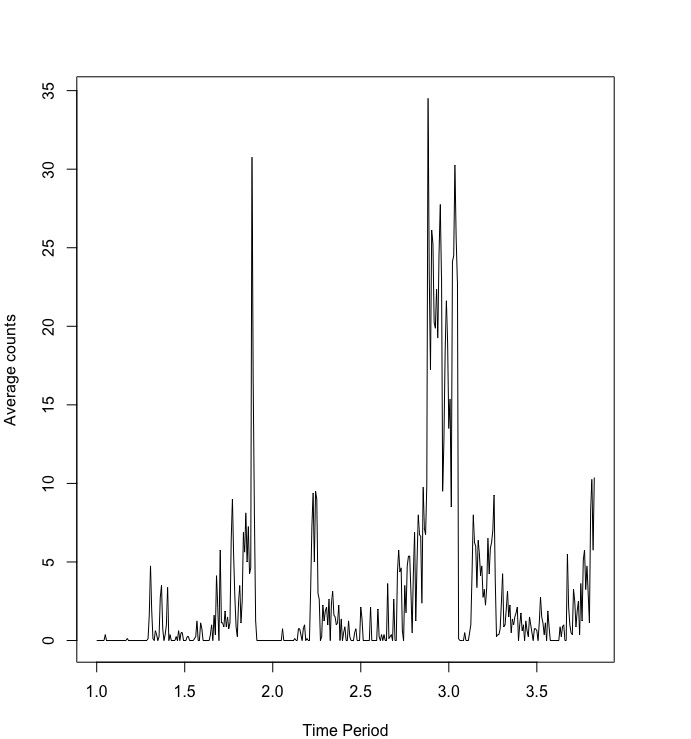
\includegraphics{VisualizeFP.jpeg}
\caption{Initial Visualization}
\end{figure}

Graph1: Orlando female non-gravid mosquito locomotor activity throughout
the period of four days. The average counts were collected every ten
minutes. The time period has been set to encompass a full 24 hour day.

\begin{figure}
\centering
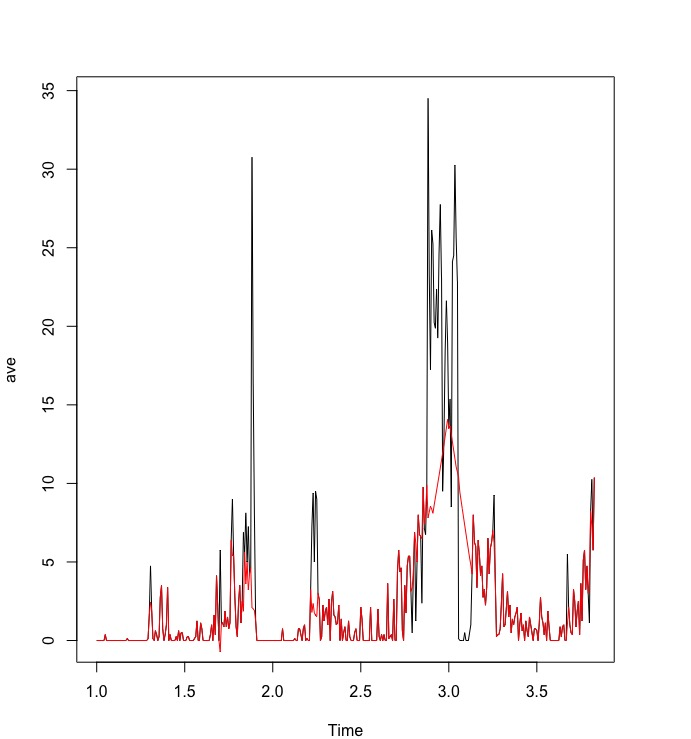
\includegraphics{RemoveOutliersFP.jpeg}
\caption{Identifying and Replacing Outliers}
\end{figure}

Graph2: Removal of any outliers from Graph1 (Orlando time series) that
could bias the model by skewing statistical summaries.

\begin{figure}
\centering
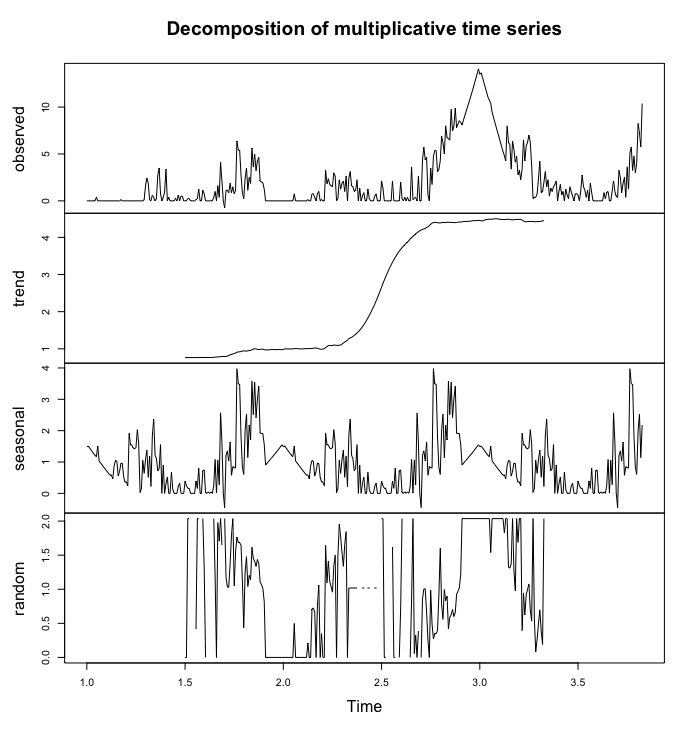
\includegraphics{DECOMPfp.png}
\caption{Decomposition of Multiplicative Time Series}
\end{figure}

Graph3: This deconstruction of the time series of Graph1 (Orlando time
series) separates the time series into the seasonal, trend and irregular
components. The Seasonal component refers to fluctuations in the data
related to daily Light:Dark cycles. Trend component is the overall
pattern of the series. It consists of decreasing or increasing patterns
that are not seasonal. This is estimated using moving averages.The part
of the series that can't be attributed to the seasonal or trend
components is referred to as residual or error.

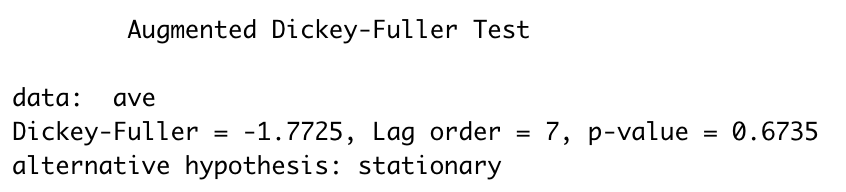
\includegraphics{ADFinal.png} The augmented Dickey-Fuller (ADF) was used
as a formal statistical test for stationarity. The null hypothesis
assumes that the series is non-stationary. ADF procedure tests whether
the change in Y can be explained by lagged value and a linear trend.
Here, he lagged value to the change in Y is non-significant and there is
a presence of a trend component, the series is non-stationary and null
hypothesis will not be rejected. This means that statistical properties
such as the mean, variance and autocorrelation are not constant over
time. Because of this, a differenced the time series was also tested
with ADF for the differenced time series had a p-value of 0.01. the
Kwiatkowski-Phillips-Schmidt-Shin (KPSS) test was also used to identify
trend-stationarity in the series, but with a p-value of 0.01, we reject
the null hypothesis, series is not stationary. There were multiple steps
of differencing taken. First-differencing the time series removed the
linear trend (i.e., differences=1); twice-differencing removed the
quadratic trend (i.e., differences=2). In addition, when
first-differencing the time series at a lag equal to the period, it
removed a seasonal trend (e.g., set lag=144 for daily collected data).

\begin{figure}
\centering
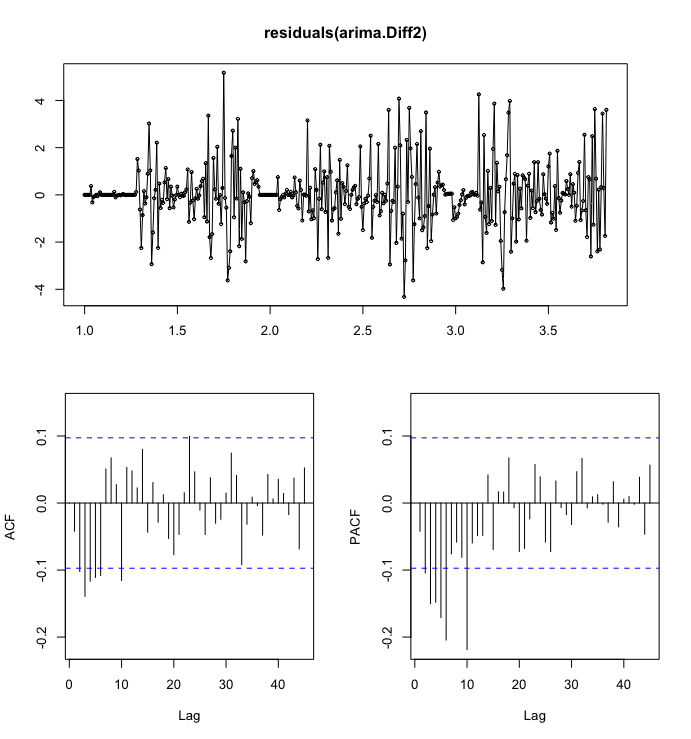
\includegraphics{ResidualsFP.png}
\caption{Residuals}
\end{figure}

Graph4: Residuals plots show a smaller error range, more or less
centered around 0. There is a clear pattern present in ACF/PACF and
model residuals plots repeating at lag 10. This suggests that our model
may be better off with a different specification, such as p = 10 or q =
10.

\begin{figure}
\centering
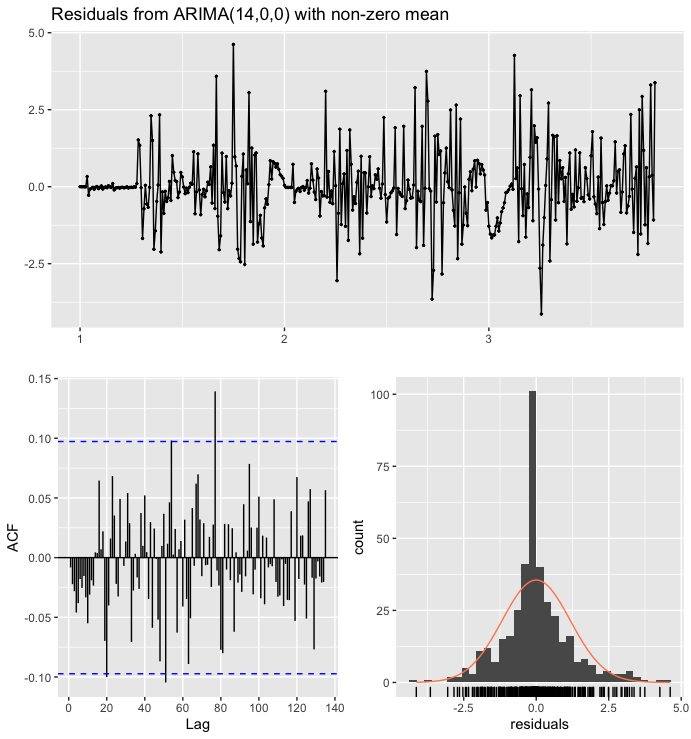
\includegraphics{AdjustResiduals.png}
\caption{Adjusted Residuals}
\end{figure}

Graph5: After increasing the lag max to 140, the best model with the
lowest AIC produced.

\begin{figure}
\centering
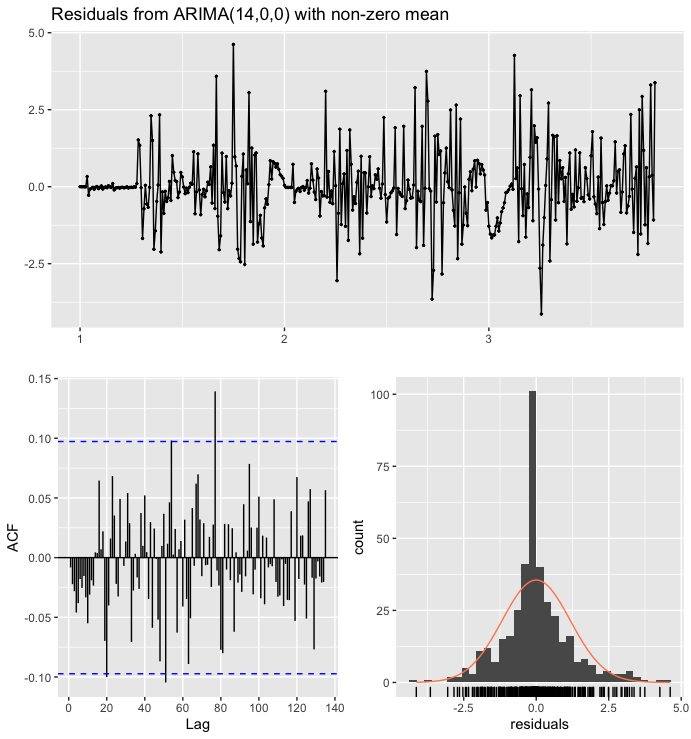
\includegraphics{ResidualsARIMA.png}
\caption{ResidualsARIMA}
\end{figure}

Graph6: The Ljung-Box test of independence at all lags up to the one
specified was conducted. Testing the ``overall'' randomness based on a
number of lags as a portmanteau test, that the residuals from the ARIMA
model have no autocorrelation. In this case the p-value was 0.3458,
confirming no significant difference from white noise.

\begin{figure}
\centering
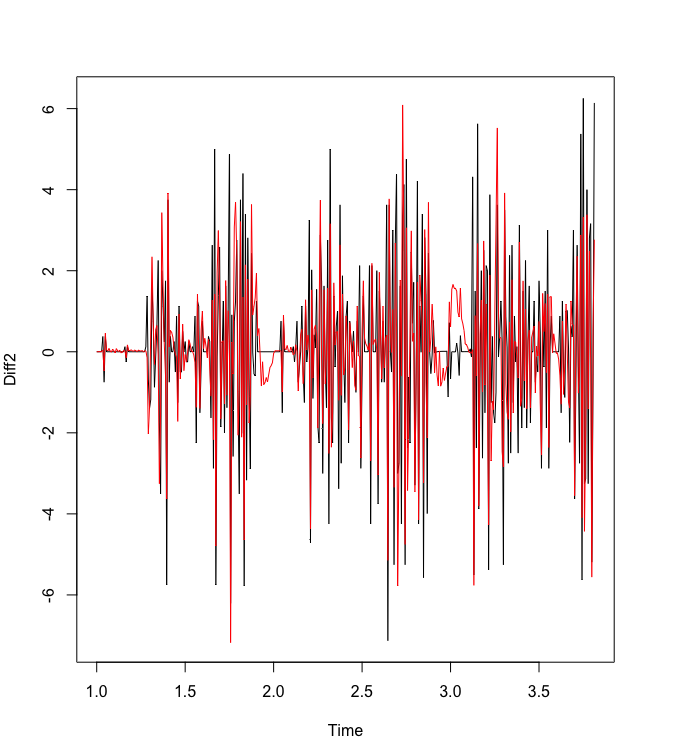
\includegraphics{TempDynFP.png}
\caption{tTemporal dynamics}
\end{figure}

Graph7: Temporal dynamics of the differenced data set for Orlando female
locomotor activity.

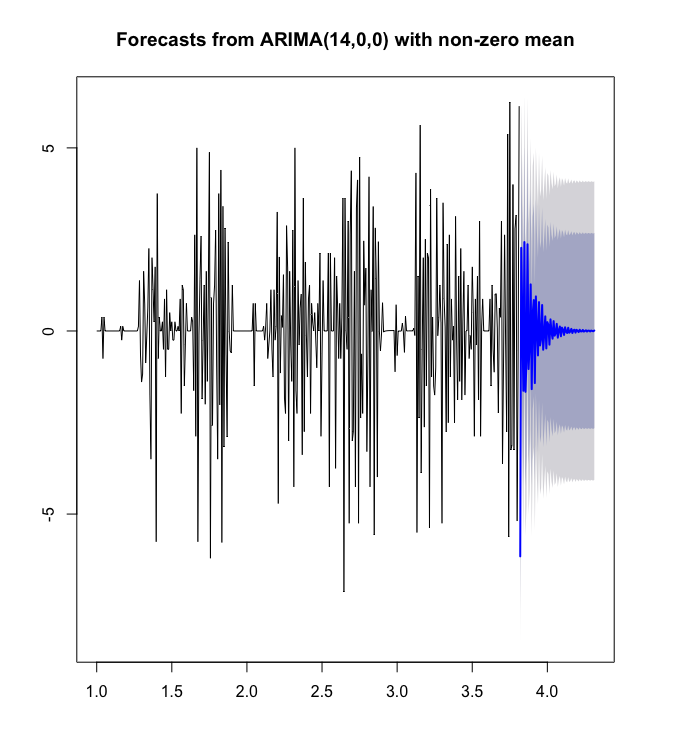
\includegraphics{Forecast.png} Graph8: Potential forecast of temporal
dynamics for Orlando female mosquitoes over the course of the next time
period using the ARIMA model.

\hypertarget{discussion}{%
\section{Discussion:}\label{discussion}}

Unfortunately, due to laboratory constraints on data production, only
Orlando female mosquitoes were able to be run and analyzed for the
purposes of this study. The study however still elucidated varying
components of this time series. For example, there seems to be a trend
of increase activity from the second to the third day in mosquitoes
within the LAM monitor. This was an issue for the ARIMA model, and steps
were taken to ensure the trends would be removed for the model to be
fitted into the data set. There also visually seems to be a seasonal
trend shown in the decomposition possibly due to the specie's diurnal
circadian rhythm for host-seeking, mating and oviposition activities. It
was only after multiple steps of differencing taken that a forecast was
achieved as an end product. This suggests there are many factors coming
into play in mosquito locomotor activity or that an insufficient amount
of data was collected for this purpose. It is possible in the future to
conduct LAM trials for longer than the 3 day period. It seems that there
may also have been many outliers still influencing the graph trends.
This may be reduced by more rigorously removing outliers previous to
importing data, or by increasing sample size and determining if the
outliers may just be the peaks of activity. More analysis has to be done
on field samples and a comparison of decomposed data may allow for a
better view at possible differences between these mosquito populations.

\hypertarget{references}{%
\section{References:}\label{references}}

Carrasco D, Lefèeye T, Moiroux N et al.~2019. Behavioural adaptations of
mosquito vectors to insecticide control. Current Opinion in Insect
Science 34: 48-54. doi: 10.1016/j.cois.2019.03.005

Edman JD, Haeger JS. 1977. Host-feeding patterns of Florida mosquitoes
Journal of Medical Entomology 14: 477--479. doi:
10.1093/jmedent/14.4.477

Gatton ML, Chitnis N, Churcher T et al.~2013. The Importance Of mosquito
behavioural adaptations to malaria control in Africa. Evolution, 67:
1218--1230. doi: 10.1111/evo.12063

Kuno G. 2010. Early history of laboratory breeding of Aedes aegypti
(Diptera: Culicidae) focusing on the origins and use of selected
strains. Journal of Medical Entomology, 47: 957--971. doi:
10.1603/me10152

Muirhead-Thomson RC. (1960). The significance of irritability,
behaviouristic avoidance and allied phenomena in malaria eradication.
Bull. Wid Hith Org.

Vontas J, Kioulos E, Pavlidi N, Mo, et al.~2012. Insecticide resistance
in the major dengue vectors Aedes albopictus and Aedes aegypti.
Pesticide Biochemistry and Physiology, 104: 126--131.
\url{doi:10.1016/j.pestbp.2012.05.008}

Yang Y-Y, Liu Y, Teng H-J, et al.~2010. Circadian control of
permethrin-resistance in the mosquito Aedes aegypti. Journal of Insect
Physiology, 56: 1219--1223. doi: 10.1016/j.jinsphys.2010.03.028

\end{document}
